% The tasks.learn pipeline with measured stage times (pitch/data/workflow_timeline.csv). Build: latexmk -pdf pipeline.tex
\documentclass[tikz,border=4mm]{standalone}
\usepackage[T1]{fontenc}
\usepackage[scaled=0.93]{helvet}
\renewcommand{\familydefault}{\sfdefault}
\usetikzlibrary{arrows.meta,calc,positioning}

\definecolor{ink}{HTML}{0B0B0B}
\definecolor{ink2}{HTML}{52514E}
\definecolor{muted}{HTML}{898781}
\definecolor{rule}{HTML}{C3C2B7}
\definecolor{band}{HTML}{F4F4F1}
\definecolor{gpu}{HTML}{2A78D6}
\definecolor{cloud}{HTML}{EB6834}
\definecolor{cpu}{HTML}{1BAF7A}
\definecolor{person}{HTML}{52514E}

\newcommand{\chip}[2]{{\color{#1}\raisebox{-0.12ex}{\scalebox{1.5}{$\bullet$}}}\hspace{0.4mm}{\color{ink2}#2}}

\begin{document}
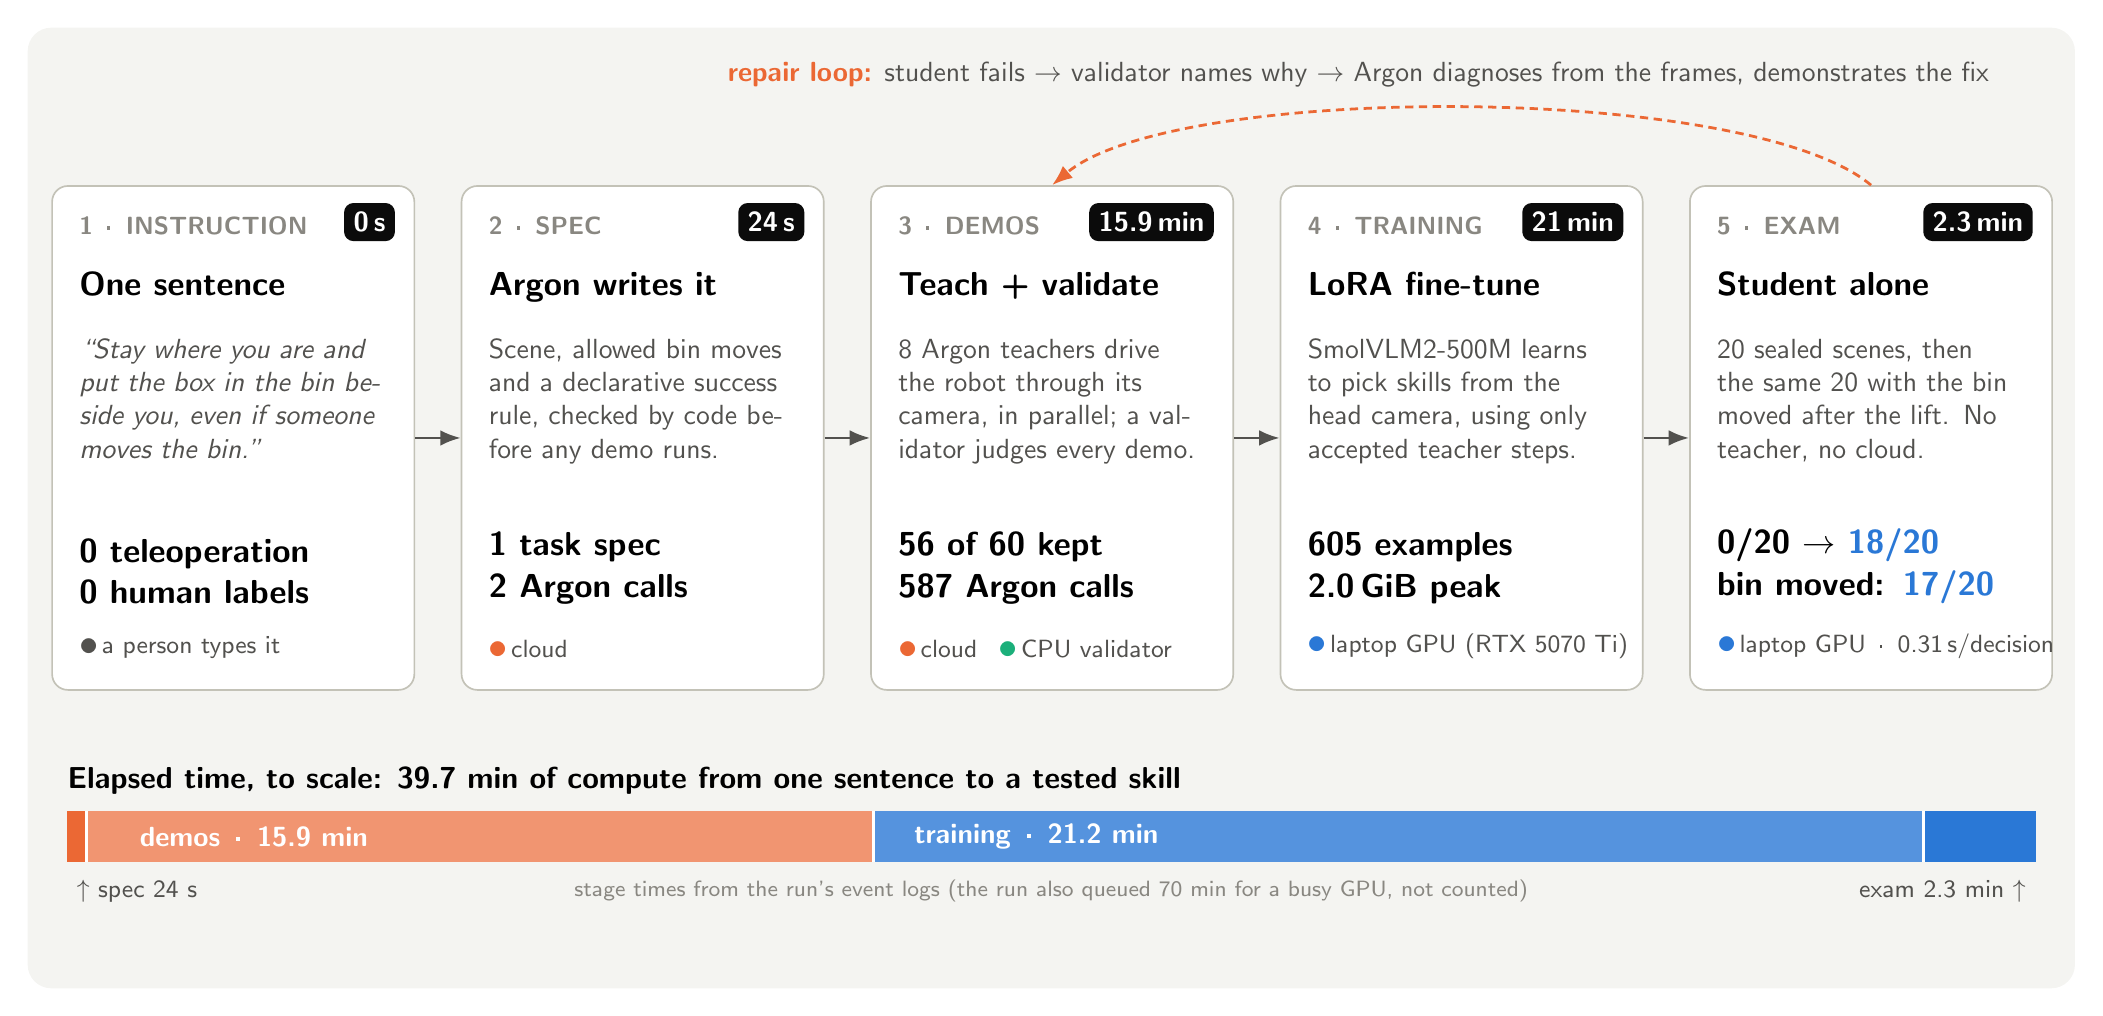
\begin{tikzpicture}[x=1mm, y=1mm,
  font=\fontsize{10}{12.4}\selectfont\color{ink},
  card/.style={draw=rule, line width=0.6pt, fill=white, rounded corners=2mm, minimum width=46mm, minimum height=52mm},
  arr/.style={-{Latex[length=2.6mm, width=2mm]}, line width=1pt, color=ink2}]

\fill[band, rounded corners=3mm] (-3,-66) rectangle (257,56);

% ---- the five stages: 70 mm tall cards, fixed zones (label, title, body, metric, where) ---------------
\foreach \i/\x in {1/0, 2/52, 3/104, 4/156, 5/208} {
  \node[card, anchor=north west, minimum height=64mm] (c\i) at (\x,36) {};
}
\newcommand{\stage}[4]{% #1 card, #2 label, #3 title, #4 time
  \node[anchor=north west, inner sep=0, font=\fontsize{9}{11}\selectfont\bfseries\color{muted}] at ($(c#1.north west)+(3.5,-4)$) {#2};
  \node[anchor=north east, inner sep=1.2mm, fill=ink, text=white, rounded corners=1.2mm, font=\fontsize{10}{12}\selectfont\bfseries] at ($(c#1.north east)+(-2.5,-2.2)$) {#4};
  \node[anchor=north west, inner sep=0, font=\fontsize{13}{15}\selectfont\bfseries] at ($(c#1.north west)+(3.5,-11)$) {#3};
}
\newcommand{\body}[2]{\node[anchor=north west, inner sep=0, text width=39mm, align=left, font=\fontsize{9.6}{12}\selectfont\color{ink2}] at ($(c#1.north west)+(3.5,-19.5)$) {#2};}
\newcommand{\metric}[2]{\node[anchor=south west, inner sep=0, text width=40mm, align=left, font=\fontsize{12.5}{15}\selectfont\bfseries] at ($(c#1.south west)+(3.5,11)$) {#2};}
\newcommand{\where}[2]{\node[anchor=south west, inner sep=0, font=\fontsize{9}{11}\selectfont] at ($(c#1.south west)+(3.5,4)$) {#2};}

\stage{1}{1 \,·\, INSTRUCTION}{One sentence}{0\,s}
\body{1}{\itshape ``Stay where you are and put the box in the bin beside you, even if someone moves the bin.''}
\metric{1}{0 teleoperation\\0 human labels}
\where{1}{\chip{person}{a person types it}}

\stage{2}{2 \,·\, SPEC}{Argon writes it}{24\,s}
\body{2}{Scene, allowed bin moves and a declarative success rule, checked by code before any demo runs.}
\metric{2}{1 task spec\\2 Argon calls}
\where{2}{\chip{cloud}{cloud}}

\stage{3}{3 \,·\, DEMOS}{Teach + validate}{15.9\,min}
\body{3}{8 Argon teachers drive the robot through its camera, in parallel; a validator judges every demo.}
\metric{3}{56 of 60 kept\\587 Argon calls}
\where{3}{\chip{cloud}{cloud} \enspace \chip{cpu}{CPU validator}}

\stage{4}{4 \,·\, TRAINING}{LoRA fine-tune}{21\,min}
\body{4}{SmolVLM2-500M learns to pick skills from the head camera, using only accepted teacher steps.}
\metric{4}{605 examples\\2.0\,GiB peak}
\where{4}{\chip{gpu}{laptop GPU (RTX 5070 Ti)}}

\stage{5}{5 \,·\, EXAM}{Student alone}{2.3\,min}
\body{5}{20 sealed scenes, then the same 20 with the bin moved after the lift. No teacher, no cloud.}
\metric{5}{0/20 $\rightarrow$ \textcolor{gpu}{18/20}\\bin moved: \textcolor{gpu}{17/20}}
\where{5}{\chip{gpu}{laptop GPU \,·\, 0.31\,s/decision}}

\foreach \a/\b in {1/2, 2/3, 3/4, 4/5} { \draw[arr] (c\a.east) -- (c\b.west); }

% ---- the repair loop (mom run) -----------------------------------------------------------------------
\draw[arr, dash pattern=on 3pt off 2pt, color=cloud] (c5.north) to[out=140, in=40, looseness=0.5] (c3.north);
\node[font=\fontsize{9.6}{11.6}\selectfont\color{ink2}, fill=band, inner sep=1mm] at (166,50)
  {\textcolor{cloud}{\textbf{repair loop:}} student fails $\rightarrow$ validator names why $\rightarrow$ Argon diagnoses from the frames, demonstrates the fix};

% ---- elapsed time, to scale ---------------------------------------------------------------------------
% stage seconds: spec 23.5, demos 952.7, training 1271.7, exam 135.9; total 2383.8 s = 39.7 min; bar 250 mm
\def\scale{0.10487} % mm per second = 250 / 2383.8
\coordinate (t0) at (2,-50);
\node[anchor=south west, inner sep=0, font=\fontsize{10.5}{12.5}\selectfont\bfseries] at ($(t0)+(0,8.5)$) {Elapsed time, to scale: 39.7 min of compute from one sentence to a tested skill};
\fill[color=cloud]            (t0) rectangle ++(23.5*\scale, 6.5);
\fill[color=cloud!70]         ($(t0)+(23.5*\scale,0)$) rectangle ++(952.7*\scale, 6.5);
\fill[color=gpu!80]           ($(t0)+(976.2*\scale,0)$) rectangle ++(1271.7*\scale, 6.5);
\fill[color=gpu]              ($(t0)+(2247.9*\scale,0)$) rectangle ++(135.9*\scale, 6.5);
\foreach \s in {23.5, 976.2, 2247.9} { \draw[white, line width=1pt] ($(t0)+(\s*\scale,0)$) -- ++(0,6.5); }
\node[anchor=west, text=white, font=\fontsize{10}{12}\selectfont\bfseries] at ($(t0)+(8,3.25)$) {demos \,·\, 15.9 min};
\node[anchor=west, text=white, font=\fontsize{10}{12}\selectfont\bfseries] at ($(t0)+(976.2*\scale+4,3.25)$) {training \,·\, 21.2 min};
\node[anchor=north west, font=\fontsize{9}{11}\selectfont\color{ink2}] at ($(t0)+(0,-1)$) {$\uparrow$ spec 24 s};
\node[anchor=north east, font=\fontsize{9}{11}\selectfont\color{ink2}] at ($(t0)+(250,-1)$) {exam 2.3 min $\uparrow$};
\node[anchor=north, font=\fontsize{8.5}{10}\selectfont\color{muted}] at ($(t0)+(125,-1)$) {stage times from the run's event logs (the run also queued 70 min for a busy GPU, not counted)};
\end{tikzpicture}
\end{document}
